\onecolumn
\noindent{\small\textbf{MATEMÁTICA E SUAS TECNOLOGIAS}}

\noindent\textbf{Questões \ref{mat-first} a \ref{mat-last}} %arrumar o número

\questao \label{mat-first} %(ENEM - 2020)
Um administrador resolve estudar o lucro de sua empresa e, para isso, traça o gráfico da receita 
e do custo de produção de seus itens, em real, em função da quantidade de itens produzidos.

\begin{center}
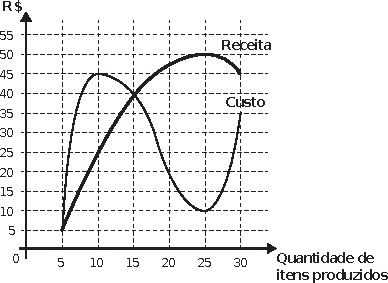
\includegraphics[width=.4\textwidth]{subareas/matematica/enem_2020-136-grafico.pdf}
\end{center}

O lucro é determinado pela diferença: Receita – Custo.

O gráfico que representa o lucro dessa empresa, em função da quantidade de itens produzidos, é

\begin{alternativas}
\setlength{\columnseprule}{0pt}
\setlength{\columnsep}{6mm}
\begin{multicols}{2}
  \item \parbox{\linewidth}{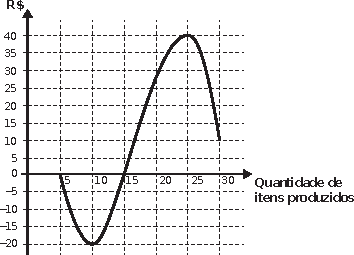
\includegraphics[width=.35\textwidth]{subareas/matematica/enem_2020-136-A.pdf}}
  \item \parbox{\linewidth}{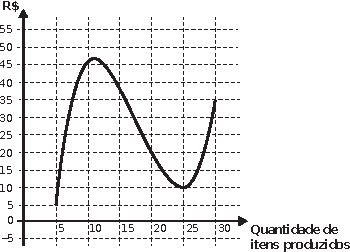
\includegraphics[width=.35\textwidth]{subareas/matematica/enem_2020-136-D.pdf}}
  \item \parbox{\linewidth}{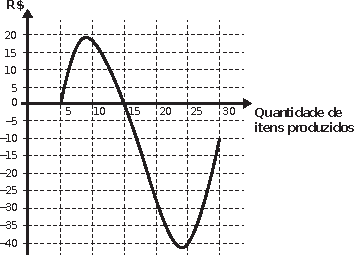
\includegraphics[width=.35\textwidth]{subareas/matematica/enem_2020-136-B.pdf}}
  \item \parbox{\linewidth}{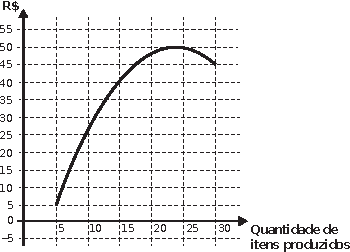
\includegraphics[width=.35\textwidth]{subareas/matematica/enem_2020-136-E.pdf}}
  \item \parbox{\linewidth}{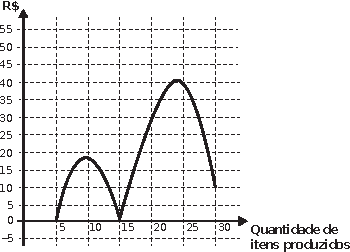
\includegraphics[width=.35\textwidth]{subareas/matematica/enem_2020-136-C.pdf}}
\end{multicols}
\end{alternativas}


\twocolumn

\questao %(ENEM - 2020)
Um motociclista planeja realizar uma viagem cujo
destino fica a 500 km de sua casa. Sua moto consome
5 litros de gasolina para cada 100 km rodados, e o
tanque da moto tem capacidade para 22 litros. Pelo
mapa, observou que no trajeto da viagem o último posto
disponível para reabastecimento, chamado Estrela, fica a
80 km do seu destino. Ele pretende partir com o tanque
da moto cheio e planeja fazer somente duas paradas para
reabastecimento, uma na ida e outra na volta, ambas no
posto Estrela. No reabastecimento para a viagem de ida,
deve considerar também combustível suficiente para se
deslocar por 200 km no seu destino.

A quantidade mínima de combustível, em litro, que
esse motociclista deve reabastecer no posto Estrela na
viagem de ida, que seja suficiente para fazer o segundo
reabastecimento, é

\begin{alternativas}
\item 13
\item 14
\item 17
\item 18
\item 21
\end{alternativas}

\questao
Uma administração municipal encomendou a pintura
de dez placas de sinalização para colocar em seu pátio
de estacionamento.

O profissional contratado para o serviço inicial
pintará o fundo de dez placas e cobrará um valor de
acordo com a área total dessas placas. O formato
de cada placa é um círculo de diâmetro $d = 40$ cm,
que tangencia lados de um retângulo, sendo que
o comprimento total da placa é $h = 60$ cm, conforme
ilustrado na figura. Use $3,14$ como aproximação para $\pi$.

\begin{center}

\includegraphics[width=.2\textwidth]{subareas/matematica/enem_2019-151-desenho.pdf}
\end{center}

Qual é a soma das medidas das áreas, em centímetros
quadrados, das dez placas?

\begin{alternativas}
\item 16 628
\item 22 280
\item 28 560
\item 41 120
\item 66 240
\end{alternativas}

\questao
O dono de um restaurante situado às margens de
uma rodovia percebeu que, ao colocar uma placa de
propaganda de seu restaurante ao longo da rodovia, as
vendas aumentaram. Pesquisou junto aos seus clientes
e concluiu que a probabilidade de um motorista perceber
uma placa de anúncio é $\displaystyle \frac{1}{2}$.
Com isso, após autorização
do órgão competente, decidiu instalar novas placas com
anúncios de seu restaurante ao longo dessa rodovia, de
maneira que a probabilidade de um motorista perceber
pelo menos uma das placas instaladas fosse superior
a $\displaystyle \frac{99}{100}$.

A quantidade mínima de novas placas de propaganda a
serem instaladas é

\begin{alternativas}
\item 99
\item 51
\item 50
\item 6
\item 1
\end{alternativas}

\questao
O colesterol total de uma pessoa é obtido pela
soma da taxa do seu “colesterol bom” com a taxa do
seu “colesterol ruim”. Os exames periódicos, realizados
em um paciente adulto, apresentaram taxa normal
de “colesterol bom”, porém, taxa do “colesterol ruim”
(também chamado LDL) de 280 mg/dL.

O quadro apresenta uma classificação de acordo com
as taxas de LDL em adultos.

\begin{center}
\begin{tabular}{|c|c|}
\hline
\multicolumn{2}{|c|}{\textbf{Taxa de LDL (mg/dL)}} \\
\hline
Ótima & Menor do que 100 \\
\hline
Próxima de ótima & De 100 a 129 \\
\hline
Limite & De 130 a 159 \\
\hline
Alta & De 160 a 189 \\
\hline
Muito alta & 190 ou mais \\
\hline
\end{tabular}
\end{center}

%\begin{flushright}
%\small Disponível em: www.minhavida.com.br. Acesso em: 15 out. 2015 (adaptado)
%\end{flushright}

O paciente, seguindo as recomendações médicas sobre estilo de vida e alimentação,
realizou o exame logo após o primeiro mês, e a taxa de LDL reduziu em $25\%$.
No mês seguinte, realizou novo exame e constatou uma redução de mais $20\%$ na taxa de LDL.

De acordo com o resultado do segundo exame, a classificação da taxa de LDL do paciente é

\begin{alternativas}
\item ótima
\item próxima de ótima
\item limite
\item alta
\item muito alta
\end{alternativas}

\questao
O Índice de Desenvolvimento Humano (IDH) é uma
medida usada para classificar os países pelo seu grau
de desenvolvimento. Para seu cálculo, são levados em
consideração a expectativa de vida ao nascer, tempo de
escolaridade e renda per capita, entre outros. O menor
valor deste índice é zero e o maior é um. Cinco países
foram avaliados e obtiveram os seguintes índices de
desenvolvimento humano: o primeiro país recebeu um
valor $X$, o segundo $\sqrt{X}$, o terceiro $\displaystyle X^{\frac{1}{3}}$,
o quarto $X^2$ e o último $X^3$. Nenhum desses países zerou ou atingiu o
índice máximo.

Qual desses países obteve o maior IDH?

\begin{alternativas}
\item O primeiro
\item O segundo
\item O terceiro
\item O quarto
\item O quinto
\end{alternativas}

\questao
Uma empresa tem diversos funcionários. Um deles
é o gerente, que recebe R\$ 1 000,00 por semana.
Os outros funcionários são diaristas. Cada um deles
trabalha 2 dias por semana, recebendo R\$ 80,00 por
dia trabalhado.

Chamando de $X$ a quantidade total de funcionários
da empresa, a quantia $Y$, em reais, que esta empresa
gasta semanalmente para pagar seus funcionários é
expressa por
\begin{alternativas}
\item $Y = 80X + 920$
\item $Y = 80X + 1000$
\item $Y = 80X + 1080$
\item $Y = 160X + 840$
\item $Y = 160X + 1000$
\end{alternativas}

\questao
Pesquisadores da Universidade de Tecnologia
de Viena, na Áustria, produziram miniaturas de
objetos em impressoras 3D de alta precisão. Ao
serem ativadas, tais impressoras lançam feixes de
laser sobre um tipo de resina, esculpindo o objeto
desejado. O produto final da impressão é uma
escultura microscópica de três dimensões, como
visto na imagem ampliada.

\begin{center}
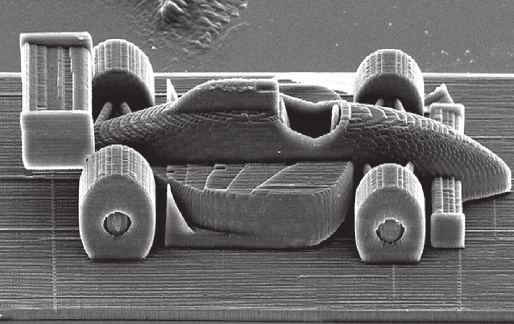
\includegraphics[width=.48\textwidth]{subareas/matematica/enem_2020-147-foto.pdf}
\end{center}

A escultura apresentada é uma miniatura de
um carro de Fórmula 1, com 100 micrômetros de
comprimento. Um micrômetro é a milionésima parte
de um metro.

Usando notação científica, qual é a representação do
comprimento dessa miniatura, em metro?

\begin{alternativas}
\item $1,0 \times 10^{-1}$
\item $1,0 \times 10^{-3}$
\item $1,0 \times 10^{-4}$
\item $1,0 \times 10^{-6}$
\item $1,0 \times 10^{-7}$
\end{alternativas}

\questao
Construir figuras de diversos tipos, apenas
dobrando e cortando papel, sem cola e sem tesoura, é
a arte do \textit{origami} (\textit{ori} = dobrar; \textit{kami} = papel), que tem
um significado altamente simbólico no Japão. A base
do origami é o conhecimento do mundo por base do
tato. Uma jovem resolveu construir um cisne usando
a técnica do \textit{origami}, utilizando uma folha de papel de
18 cm por 12 cm. Assim, começou por dobrar a folha
conforme a figura.

\begin{center}
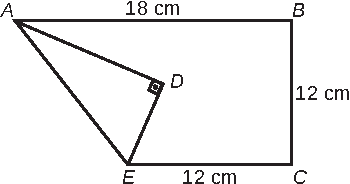
\includegraphics[width=.35\textwidth]{subareas/matematica/enem_2019-171-desenho.pdf}
\end{center}

Após essa primeira dobradura, a medida do segmento
$AE$ é

\begin{alternativas}
\item $2\sqrt{22}$ cm
\item $6\sqrt{3}$ cm
\item $12$ cm
\item $6\sqrt{5}$ cm
\item $12\sqrt{2}$ cm
\end{alternativas}

\questao \label{mat-last}
A raiva é uma doença viral e infecciosa, transmitida por mamíferos.
A campanha nacional de vacinação antirrábica tem o objetivo de controlar
a circulação do vírus da raiva canina e felina, prevenindo a raiva
humana. O gráfico mostra a cobertura (porcentagem de vacinados) da campanha, 
em cães, nos anos de 2013, 2015 e 2017, no município de Belo Horizonte,
em Minas Gerais. Os valores das coberturas dos anos de 2014 e 2016 não estão
informados no gráfico e deseja-se estimá-los. Para tal, levou-se em consideração que
a variação na cobertura de vacinação da campanha antirrábica, nos períodos
de 2013 a 2015 e de 2015 a 2017, deu-se de forma linear.

\begin{center}
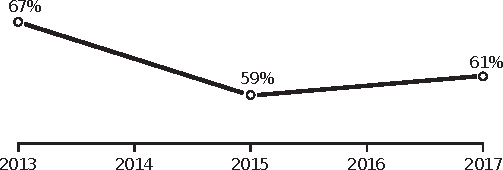
\includegraphics[width=.48\textwidth]{subareas/matematica/enem_2018-143-grafico.pdf}
\end{center}

Qual teria sido a cobertura dessa campanha no ano de 2014?

\begin{alternativas}
\item 62,3\%
\item 63,0\%
\item 63,0\%
\item 64,0\%
\item 65,5\%
\end{alternativas}
